\documentclass{article}\usepackage[]{graphicx}\usepackage[]{color}
%% maxwidth is the original width if it is less than linewidth
%% otherwise use linewidth (to make sure the graphics do not exceed the margin)
\makeatletter
\def\maxwidth{ %
  \ifdim\Gin@nat@width>\linewidth
    \linewidth
  \else
    \Gin@nat@width
  \fi
}
\makeatother

\definecolor{fgcolor}{rgb}{0.345, 0.345, 0.345}
\newcommand{\hlnum}[1]{\textcolor[rgb]{0.686,0.059,0.569}{#1}}%
\newcommand{\hlstr}[1]{\textcolor[rgb]{0.192,0.494,0.8}{#1}}%
\newcommand{\hlcom}[1]{\textcolor[rgb]{0.678,0.584,0.686}{\textit{#1}}}%
\newcommand{\hlopt}[1]{\textcolor[rgb]{0,0,0}{#1}}%
\newcommand{\hlstd}[1]{\textcolor[rgb]{0.345,0.345,0.345}{#1}}%
\newcommand{\hlkwa}[1]{\textcolor[rgb]{0.161,0.373,0.58}{\textbf{#1}}}%
\newcommand{\hlkwb}[1]{\textcolor[rgb]{0.69,0.353,0.396}{#1}}%
\newcommand{\hlkwc}[1]{\textcolor[rgb]{0.333,0.667,0.333}{#1}}%
\newcommand{\hlkwd}[1]{\textcolor[rgb]{0.737,0.353,0.396}{\textbf{#1}}}%
\let\hlipl\hlkwb

\usepackage{framed}
\makeatletter
\newenvironment{kframe}{%
 \def\at@end@of@kframe{}%
 \ifinner\ifhmode%
  \def\at@end@of@kframe{\end{minipage}}%
  \begin{minipage}{\columnwidth}%
 \fi\fi%
 \def\FrameCommand##1{\hskip\@totalleftmargin \hskip-\fboxsep
 \colorbox{shadecolor}{##1}\hskip-\fboxsep
     % There is no \\@totalrightmargin, so:
     \hskip-\linewidth \hskip-\@totalleftmargin \hskip\columnwidth}%
 \MakeFramed {\advance\hsize-\width
   \@totalleftmargin\z@ \linewidth\hsize
   \@setminipage}}%
 {\par\unskip\endMakeFramed%
 \at@end@of@kframe}
\makeatother

\definecolor{shadecolor}{rgb}{.97, .97, .97}
\definecolor{messagecolor}{rgb}{0, 0, 0}
\definecolor{warningcolor}{rgb}{1, 0, 1}
\definecolor{errorcolor}{rgb}{1, 0, 0}
\newenvironment{knitrout}{}{} % an empty environment to be redefined in TeX

\usepackage{alltt}
\usepackage{underscore}
\usepackage{rotating}
\usepackage{graphics}
\usepackage{graphicx}
\usepackage{subcaption}
\usepackage{latexsym}
\usepackage{color}
\usepackage{listings} % allows for importing code scripts into the tex file
\usepackage{wrapfig} % allows wrapping text around a figure
\usepackage{lipsum} % provides Latin text to fill up a page in this illustration (do not need it otherwise!)

% Approximately 1 inch borders all around
\setlength\topmargin{-.56in}
\setlength\evensidemargin{0in}
\setlength\oddsidemargin{0in}
\setlength\textwidth{6.49in}
\setlength\textheight{8.6in}

% Options for code listing; from Patrick DeJesus, October 2016
\definecolor{codegreen}{rgb}{0,0.6,0}
\definecolor{codegray}{rgb}{0.5,0.5,0.5}
\definecolor{codepurple}{rgb}{0.58,0,0.82}
\definecolor{backcolour}{rgb}{0.95,0.95,0.92}
\lstdefinestyle{mystyle}{
	backgroundcolor=\color{backcolour},   commentstyle=\color{codegreen},
	keywordstyle=\color{magenta},
	numberstyle=\tiny\color{codegray},
	stringstyle=\color{codepurple},
	basicstyle=\footnotesize,
	breakatwhitespace=false,         
	breaklines=true,                 
	captionpos=b,                    
	keepspaces=true,                 
	numbers=left,                    
	numbersep=5pt,                  
	showspaces=false,                
	showstringspaces=false,
	showtabs=false,                  
	tabsize=2
}

%"mystyle" code listing set
\lstset{style=mystyle}
%\lstset{inputpath=appendix/}


\title{Churn Rates Minimization} 
\author{Kelso Quan}
\IfFileExists{upquote.sty}{\usepackage{upquote}}{}
\begin{document} 

\maketitle
\begin{center}
\vspace{10cm}
\large{Executive Summary} \\
\qquad Churn rates is an important aspect to any financial tech or commercial company. Churning is when the customer cancels their subscription or ceases doing business with the company. The goal of this analysis is to minimize churn rates. In this analysis, complete case analysis was used. The number of observations was 27000 dropped to 8453 and the number of features used to find strong indicators of churn rate went from 31 to 28. The analysis used decision tree, random forest, discrete, real, and gentle Ada Boosting to model the best way to predict churn rates. Every model had very similar misclassification errors with the best model being a classification tree. The best features to indicate churn rates pertained to credit card information, rewards from credit cards, and user's financial information. 
\end{center}
\newpage

\section{Introduction} 

\qquad Churn rates are of interest to the Financial Tech companies and commercial businesses that rely on subscriptions and sale of services. Churning means cancellation of a subscription which is bad for the company. All companies would like to minimize their customers' churn rates to maximize profit. Churn is a binary response with a customer either churned or not churned. The data set has 31 features and 27000 observations. Given the data, the analysis tries to minimize churn rates by determining which features contribute heavily to customers cancelling their subscriptions and which model is the best. \\

\section{Methods} 

\qquad In this analysis, decision tree, discrete, real, and gentle Ada Boosting along with random forest were used. R/Rstudio was used to perform the analysis. For the boosting techniques, the data was divided into 2/3 training set and 1/3 test set with cross validation being used. For the random forest, the data was split 60\% training set and 40\% test set. tuneRF was a function used to determine how many features were optimal for the random forest model which turned out to be 5 with the minimal OOB error. For decision tree, cross validation was used to grow a large tree, then 1SE rule was applied to prune the tree into the best subtree. The data set had 31180 Na's. Due to heavy computational times, the analysis was done as a complete case analysis. After omitting observations with Na's, there were 8453 observations left in the data set. The analysis eliminated user (id), android_user, and app_web_user. User id was eliminated because it did not provide information in determining someone's churn rate. The variables android_user and app_web_user were also deleted because they were negatively correlated and binary. Being binary variables of negatively correlated variables signified that if the user was not an android_user meant the user was ios_user and if the user was not using application, then they were a web_user. 
\section{Results}
\begin{center}

\begin{table}[ht]
\centering
\caption{Table of the response variable}
\label{response}
\begin{tabular}{rr}
  \hline
 & count \\ 
  \hline 
!churn & 5239 \\ 
  churn & 3214 \\ 
   \hline
\end{tabular}
\end{table}
\end{center}

\subsection{Exploratory Data Analysis}

\qquad Table \ref{response} shows the response was binary. About 60\% of the users did not churn and 40\% of the users did churn. This proportion was used to split the training and test data for the random forest model. In addition, there were several features that were so skewed in distributions that it was better for those variables to become binary features. These features include registered_phones, deposits, withdrawal, purchase partners, purchases, cc taken, cc_disliked, cc_liked, and cc_application begin. cc is short for credit card. Furthermore, the analysis had to define type 1 and type 2 errors. Type 1, false positive, is predicting that the customers had churned when actually they had not churned. Type 2, false negative, is predicting that the customers had not churned when really they had churned. 

\begin{table}[ht]
\caption{Correlation plot of non-binary, numerical features}
\label{corrplot}
\centering
\begin{tabular}{rrrrrr}
  \hline
 & age & credit\_score & cc\_recommended & rewards\_earned & reward\_rate \\ 
  \hline
age & 1.00 & 0.02 & 0.14 & 0.13 & 0.12 \\ 
  credit\_score & 0.02 & 1.00 & 0.13 & 0.15 & 0.17 \\ 
  cc\_recommended & 0.14 & 0.13 & 1.00 & 0.89 & 0.85 \\ 
  rewards\_earned & 0.13 & 0.15 & 0.89 & 1.00 & 0.96 \\ 
  reward\_rate & 0.12 & 0.17 & 0.85 & 0.96 & 1.00 \\ 
   \hline
\end{tabular}
\end{table}

\qquad In table \ref{corrplot}, there are strong correlations between cc_recommended, rewards_earned, and reward_rate. There was little to no correlation between age and credit_score. Age and credit_score were weakly, positively correlated to cc_recommended, rewards_earned, and reward_rate features.


\subsection{Model Fitting and Results}
\qquad This analysis did a preliminary logistic regression to examine if it was a good model for the data. It did not preform well. Consequentially, the analysis progressed into a classification tree. The best split for the decision tree was purchase partners. That was followed by the features: rewards_earned, reward_rate, cc_recommended, and credit_score. But a single decision tree is not stable, so an ensemble of trees were created. 

\begin{table}[ht]
\centering
\caption{Misclassifications Error of Methods Used}
\label{misclass}
\begin{tabular}{cccc}
  \hline
 Method & False Positive & False Negative & Total Misclassifications \\ 
  \hline 
Single Tree & 15.21\% & 46.03\% & 27.10\% \\ 
  Gentle AdaBoost & 8.13\% & 68.3\% & 31\% \\ 
Real AdaBoost & 11.79\% & 58\% & 29.34\% \\
Discrete AdaBoost & 13.27\% & 55.6\% & 29.34\% \\
Random Forest & 18.49\% & 46.40\% & 29.10\% \\
   \hline
\end{tabular}
\end{table}
\end{center}
\qquad From table \ref{misclass}, the models have very similar misclassification errors. When looking at the total misclassification column, those error rates are strictly below 30\%. The best model being the single classification tree with the lowest total misclassifications. Gentle AdaBoost had the lowest false positive rates among all the models. 
\begin{figure}[h!]

  \centering
  \begin{subfigure}[b]{0.4\linewidth}
    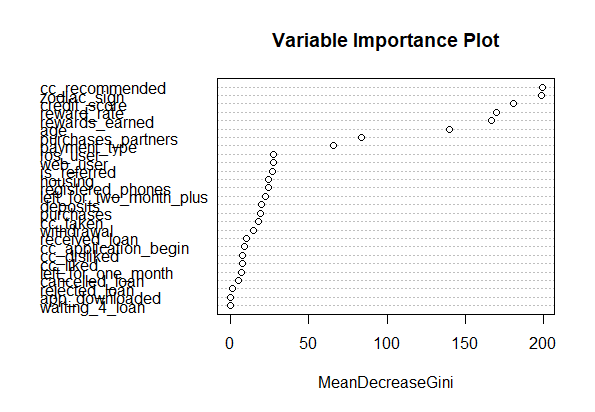
\includegraphics[width=\linewidth]{C:/Users/Kelso Quan/Documents/SchoolWork/Stat702/final/rfVarImpPlot.png}
     \caption{Random Forest}
  \end{subfigure}
  \begin{subfigure}[b]{0.4\linewidth}
    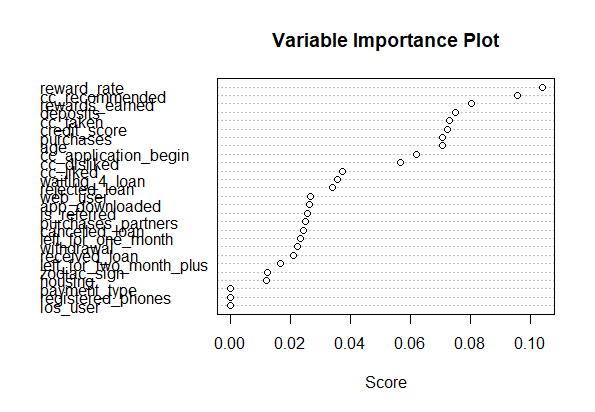
\includegraphics[width=\linewidth]{C:/Users/Kelso Quan/Documents/SchoolWork/Stat702/final/realVarPlot.png}
     \caption{Real AdaBoost}
  \end{subfigure}
  \begin{subfigure}[b]{0.4\linewidth}
    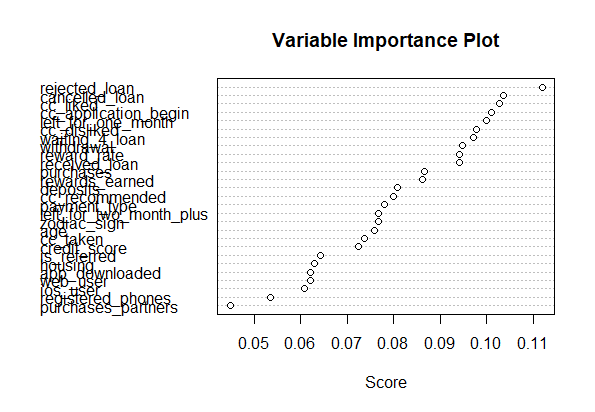
\includegraphics[width=\linewidth]{C:/Users/Kelso Quan/Documents/SchoolWork/Stat702/final/gentleVarPlot.png}
     \caption{Gentle AdaBoost}
  \end{subfigure}
  \begin{subfigure}[b]{0.4\linewidth}
    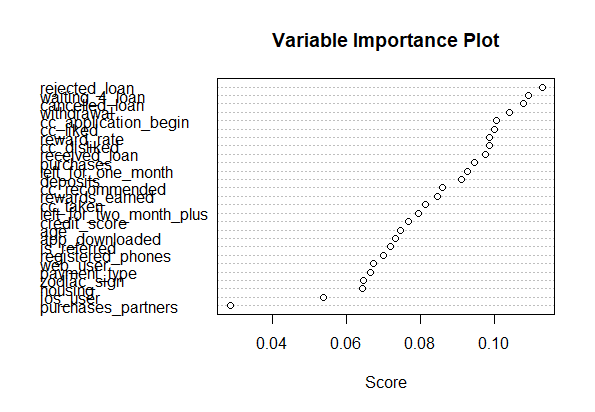
\includegraphics[width=\linewidth]{C:/Users/Kelso Quan/Documents/SchoolWork/Stat702/final/disVarPlot.png}
     \caption{Discrete AdaBoost}
     
  \end{subfigure}
  
\end{figure}

\qquad The figures (a), (b), (c), (d) shows the variable importance when it comes to predicting churn rates. Financial factors such as cc_recommended, rejected_loans, and other credit card features are significant in predicting churn rates. Any features that were closer to the right side of the importance plot were considered influential to the users' churn rate. The variables concentrated on the left side of the variable importance plot were considered less significant when it came to determining whether a customer was going to churn or not.


\section{Conclusion}
\qquad In determining an user's churn rate, it is best to consider their credit card history and financial information. cc_recommended, purchase_partners, reward_rate, and rejected_loan were of the highest variable importance when determining whether a subscriber stays in business or cancels their subscription. The analysis was slightly biased because the training-test data set ratio was different between random forest and the three methods of AdaBoost. In addition, all the models had very similar results with the decision tree being the most interpretable. The other models required variable importance plots to indicate which features contributed most to churn rates. In future analysis, the training-test data set ratio will be the same. Another constraint was the sheer amount of Na's in the data set. A considerable portion of the data was lost when complete case analysis was used rather than imputation or another method to handle missing values. Financial Tech companies should consider an user's financial history and credit card information to determine whether that user is at risk of churning.


\section{References}
Khan, Adnan \\
https://www.kaggle.com/nanda1331/churn-rate-minimization \\
stackexchange.com \\
overleaf.com \\

\newpage
\noindent \Large{{\bf Appendix: R Code}}
\lstinputlisting[language=R, caption = Churn Rates]{churnPartii.R}
\end{document}

\end{document}
